\documentclass[11pt, a4paper]{article}\usepackage[]{graphicx}\usepackage[]{xcolor}
% maxwidth is the original width if it is less than linewidth
% otherwise use linewidth (to make sure the graphics do not exceed the margin)
\makeatletter
\def\maxwidth{ %
  \ifdim\Gin@nat@width>\linewidth
    \linewidth
  \else
    \Gin@nat@width
  \fi
}
\makeatother

\definecolor{fgcolor}{rgb}{0.345, 0.345, 0.345}
\newcommand{\hlnum}[1]{\textcolor[rgb]{0.686,0.059,0.569}{#1}}%
\newcommand{\hlsng}[1]{\textcolor[rgb]{0.192,0.494,0.8}{#1}}%
\newcommand{\hlcom}[1]{\textcolor[rgb]{0.678,0.584,0.686}{\textit{#1}}}%
\newcommand{\hlopt}[1]{\textcolor[rgb]{0,0,0}{#1}}%
\newcommand{\hldef}[1]{\textcolor[rgb]{0.345,0.345,0.345}{#1}}%
\newcommand{\hlkwa}[1]{\textcolor[rgb]{0.161,0.373,0.58}{\textbf{#1}}}%
\newcommand{\hlkwb}[1]{\textcolor[rgb]{0.69,0.353,0.396}{#1}}%
\newcommand{\hlkwc}[1]{\textcolor[rgb]{0.333,0.667,0.333}{#1}}%
\newcommand{\hlkwd}[1]{\textcolor[rgb]{0.737,0.353,0.396}{\textbf{#1}}}%
\let\hlipl\hlkwb

\usepackage{framed}
\makeatletter
\newenvironment{kframe}{%
 \def\at@end@of@kframe{}%
 \ifinner\ifhmode%
  \def\at@end@of@kframe{\end{minipage}}%
  \begin{minipage}{\columnwidth}%
 \fi\fi%
 \def\FrameCommand##1{\hskip\@totalleftmargin \hskip-\fboxsep
 \colorbox{shadecolor}{##1}\hskip-\fboxsep
     % There is no \\@totalrightmargin, so:
     \hskip-\linewidth \hskip-\@totalleftmargin \hskip\columnwidth}%
 \MakeFramed {\advance\hsize-\width
   \@totalleftmargin\z@ \linewidth\hsize
   \@setminipage}}%
 {\par\unskip\endMakeFramed%
 \at@end@of@kframe}
\makeatother

\definecolor{shadecolor}{rgb}{.97, .97, .97}
\definecolor{messagecolor}{rgb}{0, 0, 0}
\definecolor{warningcolor}{rgb}{1, 0, 1}
\definecolor{errorcolor}{rgb}{1, 0, 0}
\newenvironment{knitrout}{}{} % an empty environment to be redefined in TeX

\usepackage{alltt}

\usepackage[top=1 in, bottom = 1 in, left = 1 in, right = 1 in ]{geometry}

\usepackage{amsmath, amssymb, amsfonts}
\usepackage{enumerate}
\usepackage{array}
\usepackage{multirow}
\usepackage{dingbat}
\usepackage{fontawesome5}

\title{MSMS - 106}
\author{Ananda Biswas}
\date{}
\IfFileExists{upquote.sty}{\usepackage{upquote}}{}
\begin{document}

\maketitle

\begin{center}
\textbf{Practical 02}
\end{center}


\smallpencil \hspace{0.5cm} Using the following bivariate data, obtain the following results.

\begin{table}[!htbp]
\def\arraystretch{1.5}

\begin{center}

\begin{tabular}{|>{\centering}m{2cm}|>{\centering}m{2cm}||>{\centering}m{2cm}|>{\centering\arraybackslash}m{2cm}|}

\hline

$X$ & $Y$ & $X$ & $Y$ \\

\hline

12.4 & 11.2 & 17.3 & 15.1 \\

14.3 & 12.5 & 18.4 & 16.1 \\

14.5 & 12.7 & 19.2 & 16.8 \\

14.9 & 13.1 & 17.4 & 15.2 \\

16.1 & 14.1 & 17 & 14.9 \\

16.9 & 14.8 & 17.9 & 15.6 \\

16.5 & 14.4 & 18.8 & 16.4 \\

15.4 & 13.4 & 20.3 & 17.7 \\

22.4 & 19.6 & 19.5 & 17 \\

19.4 & 16.9 & 19.7 & 17.2 \\

15.5 & 14 & 21.2 & 18.6 \\

16.7 & 14.6 & & \\

\hline

\end{tabular}
\end{center}
\end{table}

\begin{enumerate}[(a)]
  \item Karl Pearson Correlation Coefficient,
  \item Spearman's Rank Correlation Coefficient,
  \item Regression line of $Y$ on $X$,
  \item Regression line of $X$ on $Y$,
  \item Scatterplot of $X$ and $Y$ with a regression line.
\end{enumerate}

\faArrowAltCircleRight[regular] \textit{\textbf{Loading the data and previous implementations}}

\begin{knitrout}\tiny
\definecolor{shadecolor}{rgb}{0.969, 0.969, 0.969}\color{fgcolor}\begin{kframe}
\begin{alltt}
\hldef{github_path} \hlkwb{<-} \hlsng{'https://raw.githubusercontent.com/sakunisgithub/data_sets/master/msc_semester_1/sonam_madam_practical_02_data.csv'}
\hldef{our_data} \hlkwb{<-} \hlkwd{read.csv}\hldef{(github_path)}

\hlkwd{source}\hldef{(}\hlsng{'https://raw.githubusercontent.com/sakunisgithub/R-programming/master/my_implementations.R'}\hldef{)}
\end{alltt}
\end{kframe}
\end{knitrout}

\newpage

\faArrowAltCircleRight[regular] \textit{\textbf{Karl Pearson's Correlation Coefficient}} \\

Here we compute $r_{xy} = \dfrac{\text{cov } (x, y)}{\sqrt{\text{var } (x)} \cdot \sqrt{\text{var } (y)}}$, where $\text{cov } (x, y) = \dfrac{1}{n-1} \sum \limits_{i = 1}^{n} (x_i - \bar{x})(y_i - \bar{y})$.

\begin{knitrout}\footnotesize
\definecolor{shadecolor}{rgb}{0.969, 0.969, 0.969}\color{fgcolor}\begin{kframe}
\begin{alltt}
\hldef{my_covariance_function} \hlkwb{<-} \hlkwa{function}\hldef{(}\hlkwc{x}\hldef{,} \hlkwc{y}\hldef{)\{}

  \hldef{x_bar} \hlkwb{<-} \hlkwd{my_mean_function}\hldef{(x)}
  \hldef{y_bar} \hlkwb{<-} \hlkwd{my_mean_function}\hldef{(y)}

  \hldef{temp} \hlkwb{<-} \hlnum{0}
  \hlkwa{for} \hldef{(i} \hlkwa{in} \hlnum{1}\hlopt{:}\hlkwd{length}\hldef{(x)) \{}
    \hldef{temp} \hlkwb{<-} \hldef{temp} \hlopt{+} \hldef{(x[i]} \hlopt{-} \hldef{x_bar)} \hlopt{*} \hldef{(y[i]} \hlopt{-} \hldef{y_bar)}
  \hldef{\}}
  \hlkwd{return}\hldef{(temp}\hlopt{/}\hldef{(}\hlkwd{length}\hldef{(x)} \hlopt{-} \hlnum{1}\hldef{))}
\hldef{\}}
\end{alltt}
\end{kframe}
\end{knitrout}

\begin{knitrout}\footnotesize
\definecolor{shadecolor}{rgb}{0.969, 0.969, 0.969}\color{fgcolor}\begin{kframe}
\begin{alltt}
\hldef{my_correlation_function} \hlkwb{<-} \hlkwa{function}\hldef{(}\hlkwc{x}\hldef{,} \hlkwc{y}\hldef{)\{}

  \hldef{var_x} \hlkwb{<-} \hlkwd{my_sample_central_moments_function}\hldef{(x,} \hlnum{2}\hldef{)}
  \hldef{var_y} \hlkwb{<-} \hlkwd{my_sample_central_moments_function}\hldef{(y,} \hlnum{2}\hldef{)}
  \hldef{cor_xy} \hlkwb{<-} \hlkwd{my_covariance_function}\hldef{(x, y)} \hlopt{/} \hlkwd{sqrt}\hldef{(var_x} \hlopt{*} \hldef{var_y)}

  \hlkwd{return}\hldef{(cor_xy)}
\hldef{\}}
\end{alltt}
\end{kframe}
\end{knitrout}


\begin{knitrout}\footnotesize
\definecolor{shadecolor}{rgb}{0.969, 0.969, 0.969}\color{fgcolor}\begin{kframe}
\begin{alltt}
\hlkwd{my_correlation_function}\hldef{(our_data}\hlopt{$}\hldef{X, our_data}\hlopt{$}\hldef{Y)}
\end{alltt}
\begin{verbatim}
## [1] 0.9985405
\end{verbatim}
\begin{alltt}
\hlkwd{cor}\hldef{(our_data}\hlopt{$}\hldef{X, our_data}\hlopt{$}\hldef{Y,} \hlkwc{method} \hldef{=} \hlsng{"pearson"}\hldef{)}
\end{alltt}
\begin{verbatim}
## [1] 0.9985405
\end{verbatim}
\end{kframe}
\end{knitrout}

\faCheckCircle[regular] Results matched !! \\

$\bullet$ Correlation coefficient is almost 1, implying a nearly perfect linear relationship between $X$ and $Y$.
\newpage

\faArrowAltCircleRight[regular] \textit{\textbf{Spearman's Rank Correlation Coefficient}} \\

Here we compute $\rho = 1 - \dfrac{6 \sum \limits_{i = 1}^{n} d_i^2}{n(n^2 - 1)}$ where $d_i$ is the difference between the ranks of $x_i$ and $y_i$.

\begin{knitrout}\footnotesize
\definecolor{shadecolor}{rgb}{0.969, 0.969, 0.969}\color{fgcolor}\begin{kframe}
\begin{alltt}
\hldef{my_rank_correlation_function} \hlkwb{<-} \hlkwa{function}\hldef{(}\hlkwc{x}\hldef{,} \hlkwc{y}\hldef{)\{}

  \hldef{x_sorted} \hlkwb{<-} \hlkwd{my_selection_sort}\hldef{(x)}
  \hldef{y_sorted} \hlkwb{<-} \hlkwd{my_selection_sort}\hldef{(y)}

  \hldef{rank_x} \hlkwb{<-} \hlkwd{rep}\hldef{(}\hlnum{0}\hldef{,} \hlnum{23}\hldef{); rank_y} \hlkwb{<-} \hlkwd{rep}\hldef{(}\hlnum{0}\hldef{,} \hlnum{23}\hldef{)}

  \hlkwa{for} \hldef{(i} \hlkwa{in} \hlnum{1}\hlopt{:}\hlkwd{length}\hldef{(x_sorted)) \{}
    \hldef{rank_x[i]} \hlkwb{<-} \hlkwd{my_mean_function}\hldef{(}\hlkwd{which}\hldef{(x_sorted} \hlopt{==} \hldef{x[i]))}
    \hldef{rank_y[i]} \hlkwb{<-} \hlkwd{my_mean_function}\hldef{(}\hlkwd{which}\hldef{(y_sorted} \hlopt{==} \hldef{y[i]))}
  \hldef{\}}

  \hldef{sum_di_sq} \hlkwb{<-} \hlnum{0}

  \hlkwa{for} \hldef{(i} \hlkwa{in} \hlnum{1}\hlopt{:}\hlkwd{length}\hldef{(x)) \{}
    \hldef{sum_di_sq} \hlkwb{<-} \hldef{sum_di_sq} \hlopt{+} \hldef{(rank_x[i]} \hlopt{-} \hldef{rank_y[i])}\hlopt{^}\hlnum{2}
  \hldef{\}}

  \hldef{rank_corr} \hlkwb{<-} \hlnum{1} \hlopt{-} \hldef{(}\hlnum{6} \hlopt{*} \hldef{sum_di_sq)} \hlopt{/} \hldef{(}\hlkwd{length}\hldef{(x)} \hlopt{*} \hldef{(}\hlkwd{length}\hldef{(x)}\hlopt{^}\hlnum{2}\hlopt{-} \hlnum{1}\hldef{))}

  \hlkwd{return}\hldef{(rank_corr)}
\hldef{\}}
\end{alltt}
\end{kframe}
\end{knitrout}

\begin{knitrout}\footnotesize
\definecolor{shadecolor}{rgb}{0.969, 0.969, 0.969}\color{fgcolor}\begin{kframe}
\begin{alltt}
\hlkwd{my_rank_correlation_function}\hldef{(our_data}\hlopt{$}\hldef{X, our_data}\hlopt{$}\hldef{Y)}
\end{alltt}
\begin{verbatim}
## [1] 1
\end{verbatim}
\end{kframe}
\end{knitrout}

\begin{knitrout}\footnotesize
\definecolor{shadecolor}{rgb}{0.969, 0.969, 0.969}\color{fgcolor}\begin{kframe}
\begin{alltt}
\hlkwd{cor}\hldef{(our_data}\hlopt{$}\hldef{X, our_data}\hlopt{$}\hldef{Y,} \hlkwc{method} \hldef{=} \hlsng{"spearman"}\hldef{)}
\end{alltt}
\begin{verbatim}
## [1] 1
\end{verbatim}
\end{kframe}
\end{knitrout}

\faCheckCircle[regular] Results matched !! \\

$\bullet$ There is perfect agreement between $X$ and $Y$.

\newpage

\faArrowAltCircleRight[regular] \textit{\textbf{Regression equation of $Y$ on $X$}} \\

Let the regression equation of $Y$ on $X$ be $Y = aX + b$. Then $\hat{a} = r_{xy} \cdot \dfrac{s_y}{s_x}$ and $\hat{b} = \bar{y} - \hat{a} \bar{x}$.

\begin{knitrout}\footnotesize
\definecolor{shadecolor}{rgb}{0.969, 0.969, 0.969}\color{fgcolor}\begin{kframe}
\begin{alltt}
\hldef{x_bar} \hlkwb{<-} \hlkwd{my_mean_function}\hldef{(our_data}\hlopt{$}\hldef{X)}
\hldef{y_bar} \hlkwb{<-} \hlkwd{my_mean_function}\hldef{(our_data}\hlopt{$}\hldef{Y)}

\hldef{r_xy} \hlkwb{<-} \hlkwd{my_correlation_function}\hldef{(our_data}\hlopt{$}\hldef{X, our_data}\hlopt{$}\hldef{Y)}
\hldef{s_x} \hlkwb{<-} \hlkwd{sqrt}\hldef{(}\hlkwd{my_sample_central_moments_function}\hldef{(our_data}\hlopt{$}\hldef{X,} \hlnum{2}\hldef{))}
\hldef{s_y} \hlkwb{<-} \hlkwd{sqrt}\hldef{(}\hlkwd{my_sample_central_moments_function}\hldef{(our_data}\hlopt{$}\hldef{Y,} \hlnum{2}\hldef{))}

\hldef{a_yx} \hlkwb{<-} \hldef{r_xy} \hlopt{*} \hldef{(s_y} \hlopt{/} \hldef{s_x)}
\hldef{b_yx} \hlkwb{<-} \hldef{y_bar} \hlopt{-} \hldef{a_yx} \hlopt{*} \hldef{x_bar}

\hldef{b_yx; a_yx}
\end{alltt}
\begin{verbatim}
## [1] 0.434585
## [1] 0.851144
\end{verbatim}
\end{kframe}
\end{knitrout}

\begin{knitrout}\footnotesize
\definecolor{shadecolor}{rgb}{0.969, 0.969, 0.969}\color{fgcolor}\begin{kframe}
\begin{alltt}
\hldef{fit_y_on_x} \hlkwb{<-} \hlkwd{summary}\hldef{(}\hlkwd{lm}\hldef{(Y} \hlopt{~} \hldef{X,} \hlkwc{data} \hldef{= our_data))}
\hldef{fit_y_on_x}\hlopt{$}\hldef{coefficients}
\end{alltt}
\begin{verbatim}
##             Estimate Std. Error   t value     Pr(>|t|)
## (Intercept) 0.434585 0.17704865  2.454608 2.291188e-02
## X           0.851144 0.01004585 84.725922 4.148402e-28
\end{verbatim}
\end{kframe}
\end{knitrout}

\faCheckCircle[regular] Results matched !! \\

\vspace{1cm}

\faArrowAltCircleRight[regular] \textit{\textbf{Regressin equation of $X$ on $Y$}} \\

Let the regression equation of $X$ on $Y$ be $X = aY + b$. Then $\hat{a} = r_{xy} \cdot \dfrac{s_x}{s_y}$ and $\hat{b} = \bar{x} - \hat{a} \bar{y}$.

\begin{knitrout}\footnotesize
\definecolor{shadecolor}{rgb}{0.969, 0.969, 0.969}\color{fgcolor}\begin{kframe}
\begin{alltt}
\hldef{a_xy} \hlkwb{<-} \hldef{r_xy} \hlopt{*} \hldef{(s_x} \hlopt{/} \hldef{s_y)}
\hldef{b_xy} \hlkwb{<-} \hldef{x_bar} \hlopt{-} \hldef{a_xy} \hlopt{*} \hldef{y_bar}

\hldef{b_xy; a_xy}
\end{alltt}
\begin{verbatim}
## [1] -0.458156
## [1] 1.171462
\end{verbatim}
\end{kframe}
\end{knitrout}

\begin{knitrout}\footnotesize
\definecolor{shadecolor}{rgb}{0.969, 0.969, 0.969}\color{fgcolor}\begin{kframe}
\begin{alltt}
\hldef{fit_x_on_y} \hlkwb{<-} \hlkwd{summary}\hldef{(}\hlkwd{lm}\hldef{(X} \hlopt{~} \hldef{Y,} \hlkwc{data} \hldef{= our_data))}
\hldef{fit_x_on_y}\hlopt{$}\hldef{coefficients}
\end{alltt}
\begin{verbatim}
##              Estimate Std. Error   t value     Pr(>|t|)
## (Intercept) -0.458156 0.21336727 -2.147265 4.360262e-02
## Y            1.171462 0.01382649 84.725922 4.148402e-28
\end{verbatim}
\end{kframe}
\end{knitrout}

\faCheckCircle[regular] Results matched !! \\

\newpage

\faArrowAltCircleRight[regular] \textit{\textbf{Scatterplot of $X$ and $Y$ with a regression line}} \\

\begin{knitrout}\footnotesize
\definecolor{shadecolor}{rgb}{0.969, 0.969, 0.969}\color{fgcolor}\begin{kframe}
\begin{alltt}
\hlkwd{library}\hldef{(tidyverse)}
\end{alltt}
\end{kframe}
\end{knitrout}

\begin{knitrout}\footnotesize
\definecolor{shadecolor}{rgb}{0.969, 0.969, 0.969}\color{fgcolor}\begin{kframe}
\begin{alltt}
\hldef{our_data} \hlopt
  \hlkwd{ggplot}\hldef{(}\hlkwd{aes}\hldef{(}\hlkwc{x} \hldef{= X,} \hlkwc{y} \hldef{= Y))} \hlopt{+}
  \hlkwd{geom_point}\hldef{(}\hlkwc{size} \hldef{=} \hlnum{3}\hldef{,} \hlkwc{col} \hldef{=} \hlsng{"#f03608"}\hldef{)} \hlopt{+}
  \hlkwd{labs}\hldef{(}\hlkwc{title} \hldef{=} \hlsng{"Scatterplot of our data"}\hldef{)} \hlopt{+}
  \hlkwd{geom_smooth}\hldef{(}\hlkwc{method} \hldef{=} \hlsng{"lm"}\hldef{,} \hlkwc{formula} \hldef{= y} \hlopt{~} \hldef{x,} \hlkwc{level} \hldef{=} \hlnum{0.95}\hldef{)}
\end{alltt}
\end{kframe}
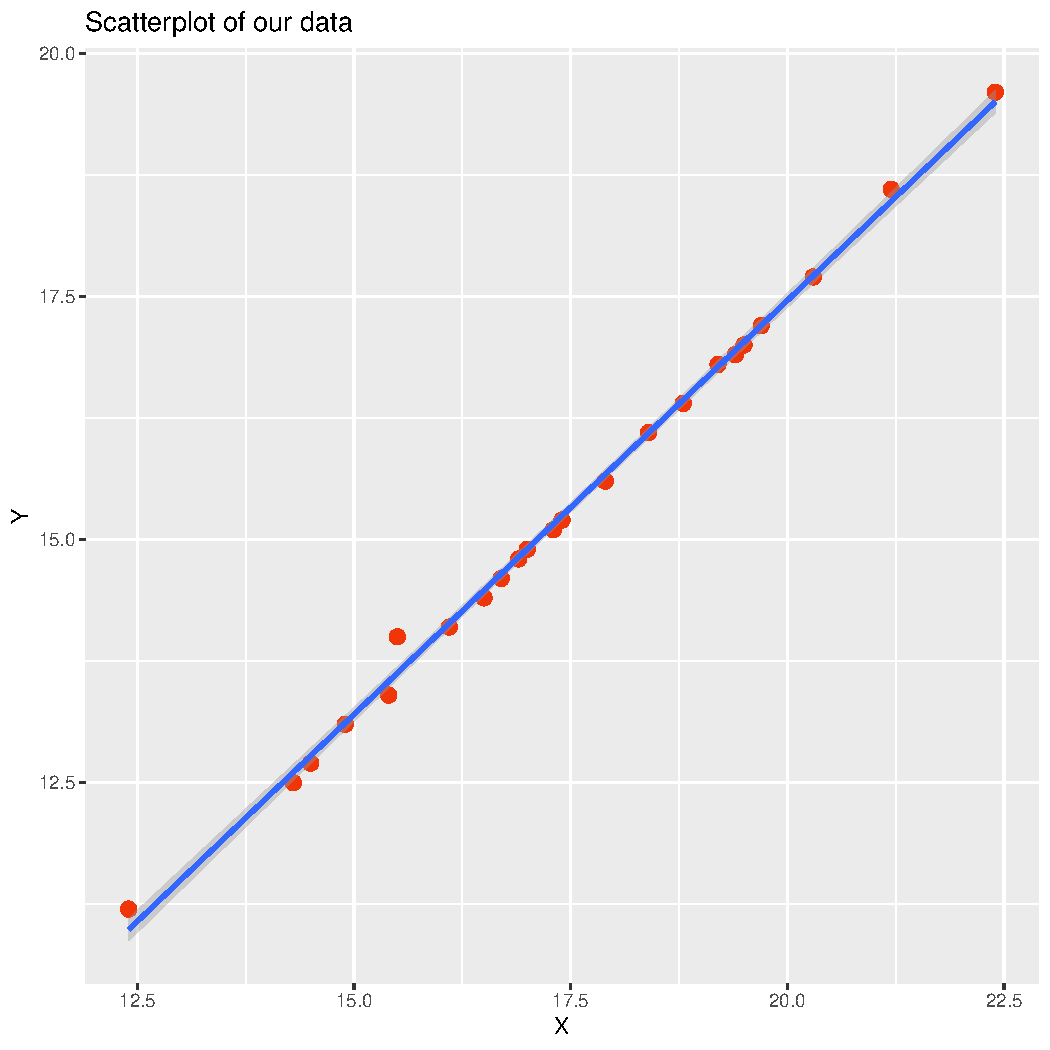
\includegraphics[width=\maxwidth]{figure/unnamed-chunk-13-1} 
\end{knitrout}

$\bullet$ An almost perfect linear relation between $X$ and $Y$ is visible.
\end{document}
